\documentclass[a4paper,12pt]{report}
\usepackage[T1]{fontenc}
\usepackage[utf8]{inputenc}
\def\magyarOptions{defaults=hu-min}
\usepackage[magyar]{babel}
\usepackage{amsthm, amssymb,amsmath,hyperref}
\usepackage{enumerate, graphicx, xcolor}

\usepackage{chngcntr}
\counterwithout{figure}{chapter}
\counterwithout{figure}{section}
\counterwithout{figure}{subsection}
%\usepackage{pgf,tikz,float}
%\usepackage{tikzlings}
%\usepackage{tikzducks}
%\usetikzlibrary{arrows}
\usepackage[nobysame]{amsrefs}
%\usepackage{amsmath}

\usepackage{geometry}
   \geometry{
   a4paper,
   total={160mm,247mm},
   left=25mm,
   top=25mm,
}

\date{today}

\linespread{1.3}

\begin{document}
\thispagestyle{empty}

\begin{center}
\vspace*{0.2cm} {\Large\bf Szegedi Tudományegyetem}
\vspace{0.3cm}

{\Large\bf Természettudományi és Informatikai Kar}
\vspace{0.3cm}

{\Large\bf Informatikai Intézet, Számítástudomány Alapjai Tanszék}
\vspace{3cm}



{\Large SZAKDOLGOZAT}

\vspace*{1.5cm}

{\LARGE\bf Tanulmányokat segítő webalkalmazás egyetemi hallgatók számára}

\vspace*{4cm}

{\large
    \begin{tabular}{c@{\hspace{2cm}}c}
        \emph{Készítette:}     &\emph{Témavezető:}\\
        \bf{Kozma Kristóf}  &\bf{Dr. Iván Szabolcs}\\
        Programtervező Informatikus BSc hallgató    & TODO\\
        &
    \end{tabular}
}

\vspace*{1,5cm}

{\Large Szeged\\ \vspace{2mm} 2024}
\end{center}


\newpage
{\Huge \bf Feladatkiírás}

\vspace{2 cm}

Az egyetemi hallgatóknak rengeteg információval kell tisztában lenniük. Látniuk kell a mintatantervbeli haladásukat, a tanulmányai átlagukat különböző ösztöndíjak tekintetében, és meg kell tervezniük az időbeosztásukat az egyetemi órák mellett, hiszen sokan ekkor kezdenek el dolgozni is. A hallgató feladata egy webalkalmazás létrehozása, ami képes könnyűvé és gördülékennyé tenni ezeket a folyamatokat, valamint átláthatóan rendszerezni a számára fontos, az egyetemmel kapcsolatos általános tudnivalókat.


\begin{abstract}
    [téma megnevezése]

    Célom egy olyan alkalmazás elkészítése volt, mely nagyban meg tudja könnyíteni az egyetemi hallgatók számára tanulmányaik követését mindennapjaik során. Ehhez az Angular nevű TypeScript keretrendszert választottam, mert ideálisnak tartom nagy alkalmazások elkészítéséhez, melyek sok, jól elkülöníthető részre tagozódnak, és összetett adatfolyamokkal dolgoznak. Ezen kívül hangsúlyt fektettem rá, hogy ne csak a Szegedi Tudományegyetem hallgatóira szabjam az alkalmazást, hanem általánossá tegyem, hogy az egész országban, de akár potenciálisan külföldön is használható legyen egyetemi hallgatók számára.
    
    Az elkészült Apollo nevű alkalmazás véleményem szerint sikeresen kielégíti ezeket az igényeket, és több egyetemi hallgató ismerősöm is megerősítette ezt.

    \textbf{Kulcsszavak:} webalkalmazás, egyetem, hallgató, Angular
\end{abstract}

\newpage

\pagebreak

\tableofcontents
\pagebreak

\chapter{Érdemi rész}
\pagenumbering{arabic}

\section{Motiváció}

Egyetemi tanulmányaim során én is sokszor éreztem azt a problémát, hogy nem tudom, hogy állok a mintatantervben, mert a Neptun és a CooSpace rendszerében nagyon nehezen elérhetők az ezzel kapcsolatos információk, és magukat a közzétett adatokat sem könnyű átlátni. Ezenkívül sokszor Excel táblában számoltam vizsgaidőszakban az átlagomat, akár tanulmányi ösztöndíjjal kapcsolatban, mert erre nem nyílt egyszerűbb mód. Valamint az órarend megtervezését is mindig nehézségnek éreztem, amikor össze kellett állítanom a sok lehetséges kurzus közül, hogy melyikeket szeretném felvenni. Ezeket a problémákat szerettem volna megoldani, amik bármelyik hallgató tanulmányai során felmerülhetnek.

\subsection{Az alkalmazás neve}

Az alkalmazásnak az Apollo nevet adtam. A Neptunhoz hasonlóan egy ókori istenről szerettem volna elnevezni. Azért Apollónra esett a választásom, mert bár legszélesebb körben a Nap, a művészetek és az íjászat isteneként ismert, ő a tudás, oktatás és fiatalság istene, valamint a zenéé és a táncé is, amik nagyon jól kapcsolódnak az egyetemistákhoz. Ezzel szerettem volna jelezni, hogy az alkalmazás az egyetemi hallgatók hétköznapjainak megkönnyítésére készült.

\section{Terület áttekintése}

A kiinduláshoz figyelembe vettem, hogy milyen alkalmazások/weboldalak érhetőek el a magyar egyetemisták számára, amik ki tudják elégíteni a bennem is felmerült igényeket, valamint felhasználói interjúkat készítettem, hogy mások, más nézőpontból is rá tudjanak világítani ezekre a nehézségekre, és képet kapjak több felhasználó igényeiről is.

\subsection{Piackutatás}

Magyarország legnagyobb egyetemi tanulmányi alkalmazása a Neptun, melyben elérhetők azok a funkciók, melyeket az Apollo is szeretne megvalósítani, csak egyik sem felhasználóbarát módon:

\begin{itemize}
    \item A mintatantervbeli haladás megtekintésére nincs mód, egyedül a teljes mintatantervet lehet megtekinteni, és azzal egyesével összehasonlítani a hallgató által már elvégzett vagy elvégzendő kurzusokat. Ugyanez a helyzet a specializációkkal is, a Neptun felülete ugyanúgy teszi lehetővé a specializációkkal való haladás megtekintését, mint a mintatantervét.
    \item A tanulmányi átlagokat megjeleníti a Neptun, azonban a hallgatónak nincs lehetősége, hogy tudjon ezekkel tervezni is. Leginkább vizsgaidőszakban releváns a hallgatók számára az átlaguk, amikor megtervezik, melyik vizsgára mennyit készüljenek, a Neptun azonban csak a vizsgaidőszak lezártával teszi láthatóvá az átlagokat, ami megakadályozza a hallgatókat, hogy a tervezéshez fel tudják használni a Neptun átlagösszesítő funkcióját.
    \item A Neptunban van órarendtervező funkció, amivel az adott tárgyhoz kötődő egyetlen kurzust hozzá lehet adni az órarendhez, ami képes lehet vizualizálni az esetleges óraütközéseket. Azonban egy nagyobb létszámú szakon, például Programtervező informatikus BSc szakon, ahol egyetlen tárgyhoz akár tíz gyakorlat is meg lehet hirdetve, nagyon nehéz eldönteni ez alapján, hogy a hallgatónak melyik a legmegfelelőbb a felsorolt órák közül. Továbbá, ha figyelembe akarja venni az egyéb, egyetemen kívüli elfoglaltságait (munka, sport, rendszeres közösségi programokra járás), azt már meg sem teheti a Neptunban, csak egy külső naptár alkalmazás segítségével.
\end{itemize}

\subsection{Felhasználói interjúk}

A felhasználói interjúk során a következő problémákat véltem felfedezni, amiben más egyetemisták is szenvednek a Neptun használata során:

\begin{itemize}
    \item Az átlagok azonnali kiszámítása fontos lenne vizsgaidőszakban. Nagyon sokan számolják egy Excel táblázatban az átlagukat, vagy akár tantárgyanként a pontszámaikat, amivel képet kaphatnak körülbelül az elkövetkező félév végi eredményeikről.
    \item A tanulmányi vagy állami ösztöndíjak feltételei sokak számára nem tiszták, és aki szeretné ezeket megkapni, és a ponthatáron van, annak szüksége lenne egy megbízható eszközre, amire hagyatkozhat a jegyeinek a kialakításakor.
    \item A mintatantervbeli haladás követése mindenkinek problémát okoz, sokan ellentmondásos információkkal is találkoznak különböző platformokon, amik alapján nehéz eldönteni, hogy pontosan hol is tartanak a diplomájuk megszerzésében.
    \item Volt, aki azt hozta fel, hogy az egyetemi szabályzat elemei, például a TVSZ egy olyan dolog, amire sokszor hivatkoznak, de annál kevesebben ismerik a pontos tartalmát. Ilyesféle szabályok és az egyetemmel kapcsolatos hasznos információmorzsák megjelenítését is szívesen fogadná egy eféle alkalmazásban.
\end{itemize}

\section{Funkcionális specifikáció}

\subsection{Funkciólista}

A saját magam, és az interjúalanyaim által megfogalmazott problémafelvetések alapján a következő főbb funkciókat vizualizáltam az alkalmazásnak:

\begin{enumerate}
    \item tanulmányi átlagok áttekintése
    \begin{enumerate}
        \item félévek hozzáadása, törlése, módosítása
        \item átlagok megtekintése (súlyozott átlag, kreditek, kreditindex, korrigált kreditindex)
        \item jegyek hozzáadása, törlése, módosítása
        \item alternatív jegyek beállítása (pl. hogyan változna az átlag egy vizsga javítása után)
        \item tanulmányi ösztöndíj számítás (az adott átlaghoz körülbelül milyen ösztöndíj járna az adott szakon)
        \item állami ösztöndíj feltételek teljesülésének jelzése
        \item vendég felhasználó is felviheti jegyeit, ami helyileg tárolódik
        \item vendég felhasználó törölheti a lokálisan eltárolt adatokat
    \end{enumerate}
    \item mintatantervbeli haladás áttekintése
    \begin{enumerate}
        \item félévek hozzáadása, törlése, módosítása
        \item teljesített tárgyak hozzáadása, törlése, módosítása
        \item tárgycsoportok megtekintése, ahol még hiányzik kredit
        \item teljesítetlen tárgycsoportok teljesítetlen tárgyainak kilistázása
    \end{enumerate}
    \item órarendtervezés
    \begin{enumerate}
        \item félévek hozzáadása, törlése, módosítása
        \item kategóriák felvitele, törlése, módosítása, órák hozzáadása kategóriákhoz
        \item órák felvitele, törlése, módosítása
        \item órarend megtekintése
        \item vendég felhasználó is felviheti óráit, ami helyileg tárolódik
        \item vendég felhasználó törölheti a lokálisan eltárolt adatokat
    \end{enumerate}
    \item autentikáció
    \begin{enumerate}
        \item vendég felhasználó tud regisztrálni és bejelentkezni
        \item bejelentkezett felhasználó tudja módosítani az adatait és beállításait
    \end{enumerate}
    \item adminisztráció: csak admin felhasználók számára
    \begin{enumerate}
        \item egyetemek hozzáadása, módosítása
        \item egyetemi karok hozzáadása, törlése, módosítása
        \item tárgyak hozzáadása adott egyetemhez, majd ezek módosítása, törlése
        \item szakok hozzáadása adott egyetemhez, majd ezek módosítása, törlése
        \item tárgyak hozzárendelése adott szakhoz, majd ezek módosítása, törlése
        \item specializációk hozzáadása adott egyetemhez, majd ezek módosítása, törlése
        \item tárgyak hozzárendelése adott specializációhoz, majd ezek módosítása, törlése
        \item korábbi évek ösztöndíjértékeinek hozzáadása adott szakhoz, majd ezek módosítása, törlése
    \end{enumerate}
    \item nyelv átállítása
\end{enumerate}

\subsection{Folyamatábra}

Egy folyamatábra segítségével terveztem meg az alkalmazás oldalait, és hogy hogyan érhetők el rajta a különböző, az előző pontban megfogalmazott funkciók.

Teljesen oválisan jelöltem az oldalakat, valamint szaggatott szegélyt adtam a dialógusablakokban elérhető funkcióknak.

\begin{figure}
    \centering
    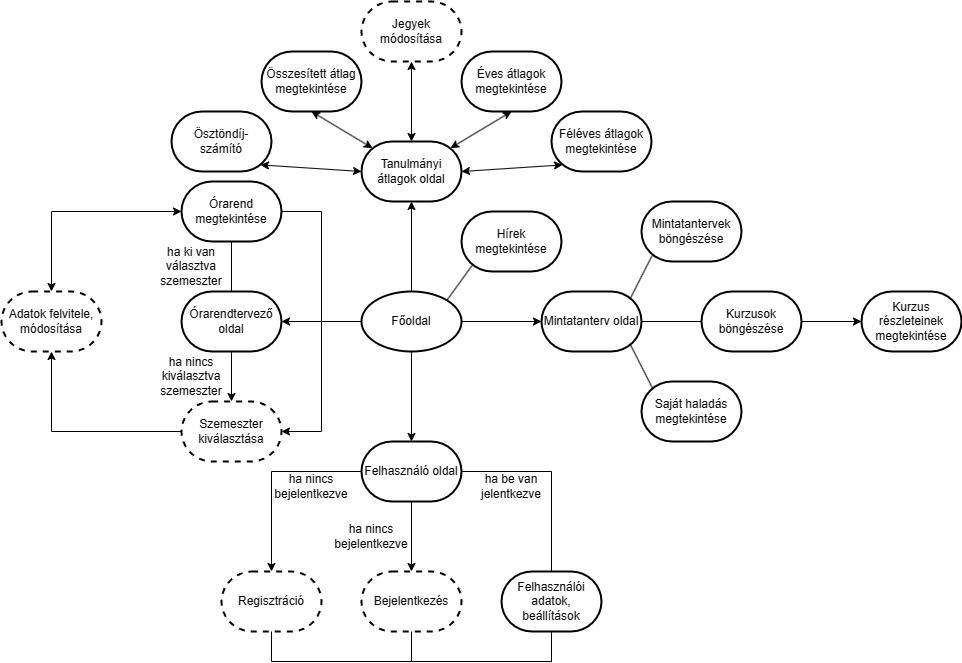
\includegraphics[width=1\linewidth]{flowchart.png}
    \caption{Folyamatábra}
\end{figure}

\section{Vizuális tervezés}

Nagy hangsúlyt fektettem az alkalmazás vizuális tervezésére, hiszen ettől nagyban függ a felhasználói élmény.

\subsection{Hangulattábla (moodboard)}

Többször is újraterveztem az alkalmazás hangulattábláját, mert nem voltam elégedett az első változatokkal. Mindenképpen szerettem volna, ha Apollón istenhez is kötődik az alkalmazás színvilága, valamint a meleg színekkel kellemesebb, otthonosabb felhasználói élményt biztosít.

\begin{figure}
    \centering
    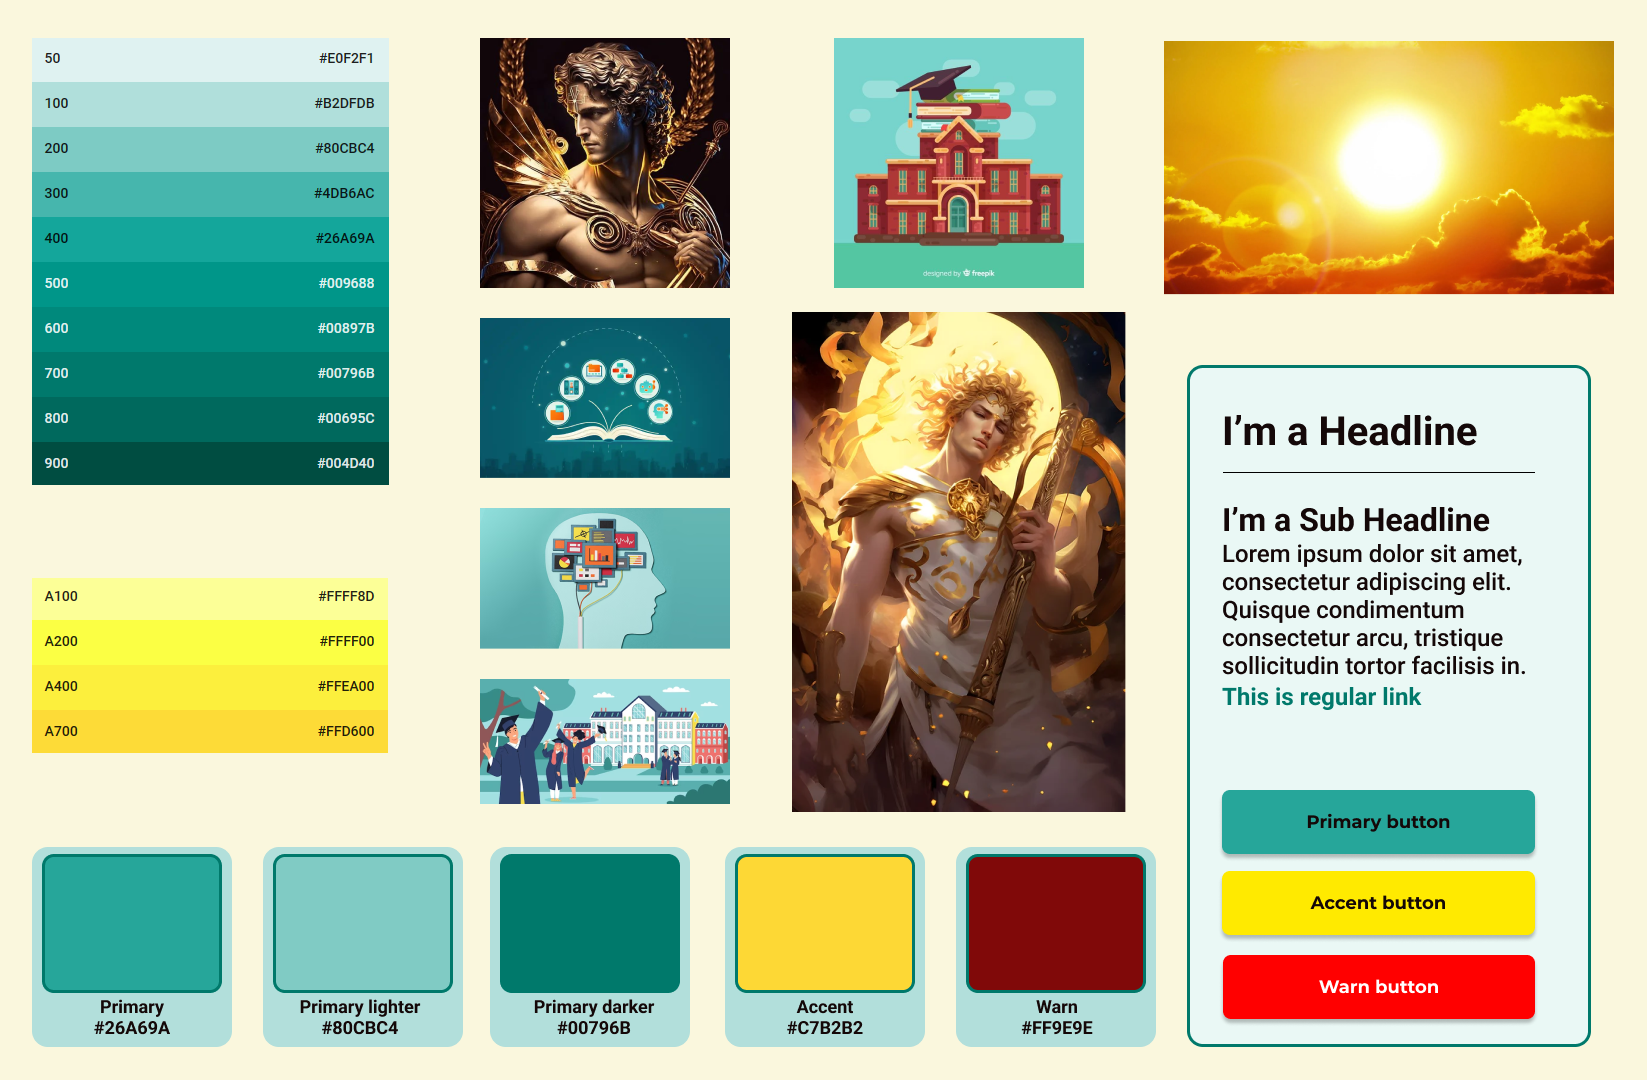
\includegraphics[width=1\linewidth]{moodboard1.png}
    \caption{Első hangulattábla}
    \label{fig:enter-label}
\end{figure}

Az első hangulattábla nem passzolt ezekhez az elképzeléseimhez, és a túl változatos színvilága nem érte el ezt az otthonosabb felhasználói élményt, ami az elsődleges célom volt.

\begin{figure}
    \centering
    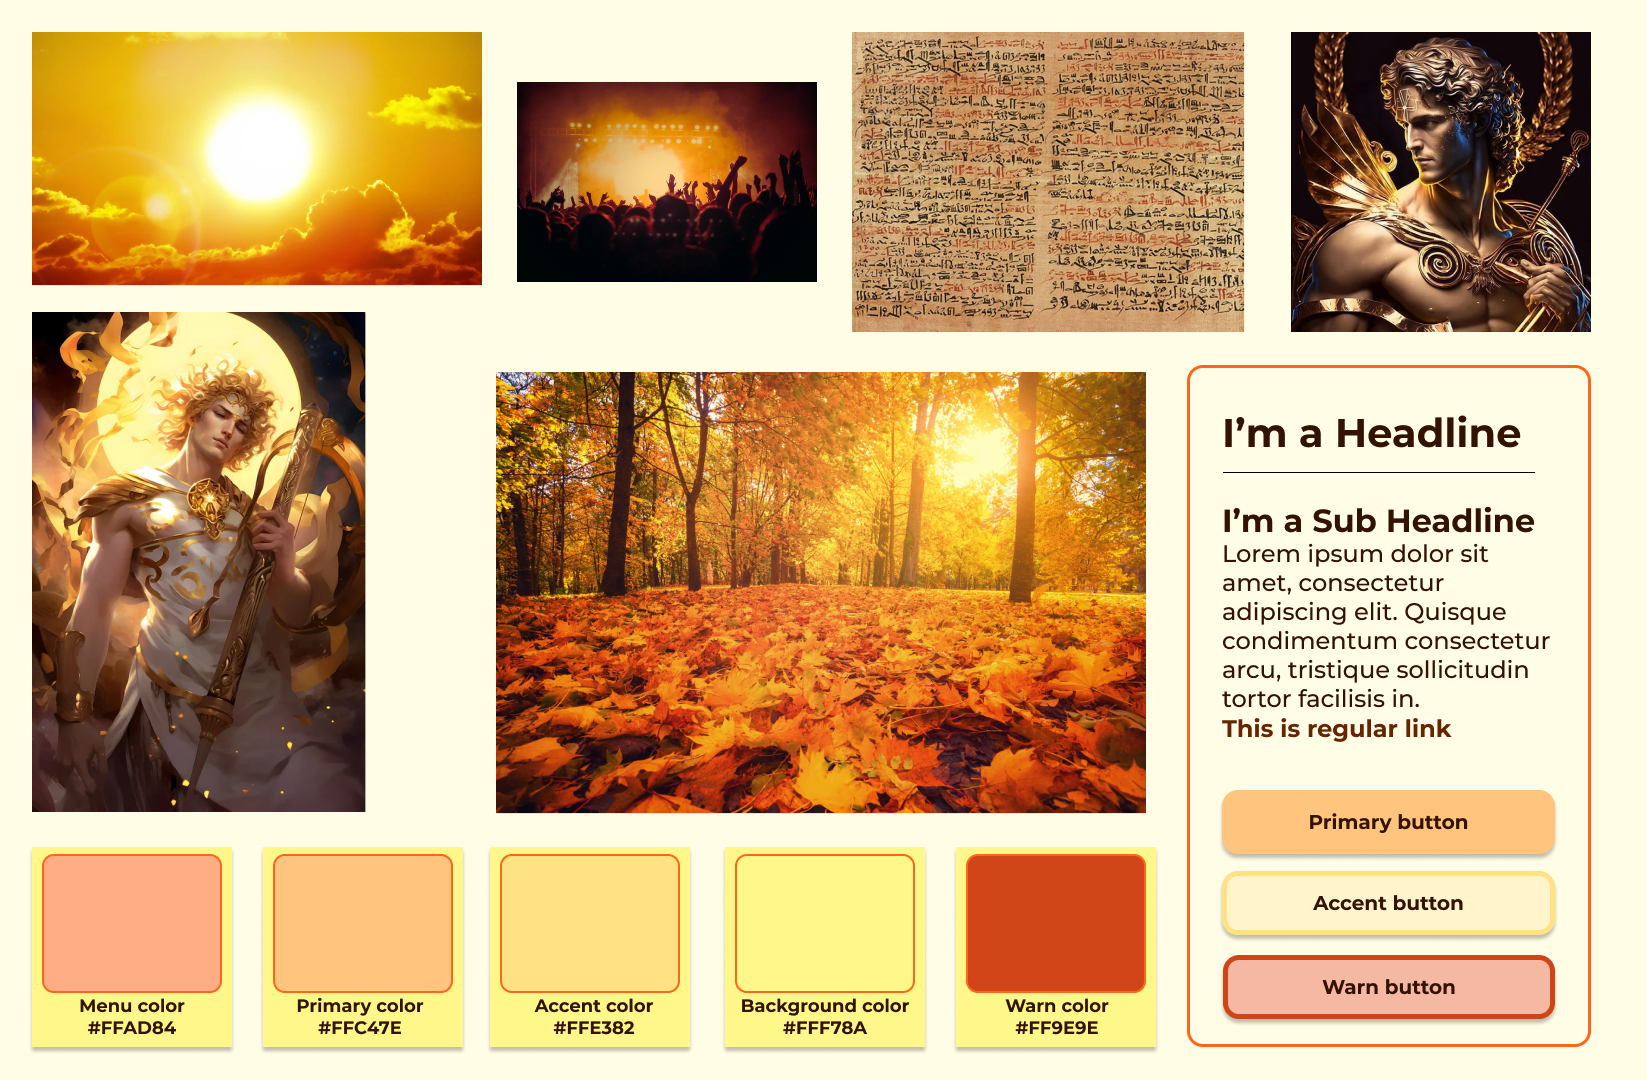
\includegraphics[width=1\linewidth]{moodboard2.png}
    \caption{Második hangulattábla}
    \label{fig:enter-label}
\end{figure}

\section{Használt technológiák}

Az alkalmazást Angularban írtam, ami egy TypeScript keretrendszer, melyet az NPM (Node Package Manager) segítségével buildelni és futtatni. 

\section{Modulok}

\section{Adatmodell}

\section{A rendszer magasszintű folyamatai, működése}

\section{Fontosabb kódrészletek}

\section{Tesztelés}

\section{Tapsztalatok, továbbfejlesztési lehetőségek}


\chapter*{Irodalomjegyzék}

\newpage
{\Huge \bf Nyilatkozat}

\addcontentsline{toc}{chapter}{Nyilatkozat}

\vspace{2 cm}

Alulírott, Kozma Kristóf, Programtervező Informatikus BSc szakos hallgató, kijelentem, hogy a szakdolgozatban ismertetettek saját munkám eredményei, és minden felhasznált, nem saját munkából származó eredmény esetén hivatkozással jelöltem annak forrását. 


\begin{flushleft}
\vspace*{1cm}
Szeged, \today
\end{flushleft}

\begin{flushright}
   \vspace*{1cm}
   \makebox[7cm]{\rule{6cm}{.4pt}}\\
   \makebox[7cm]{\emph{Kozma Kristóf}}
\end{flushright}


\newpage
{\Huge \bf Köszönetnyilvánítás}

\addcontentsline{toc}{chapter}{Köszönetnyilvánítás}

\vspace{2 cm}

Szeretnék köszönetet mondani Dr. Gazdag Zsoltnak, belső témavezetőmnek, aki mindig rendelkezésemre állt, amikor csak kérdésem volt a dolgozattal kapcsolatban, valamint Jánki Zoltánnak, aki, bár nem volt témavezetőm, rengeteg szakmai kérdésben segített munkám során.

Köszönöm a segítségét Fazekas Viviennek, aki fontos visszajelzéseket adott az alkalmazásról annak még korai fázisában.

Köszönöm továbbá Szoboszlai Leonának, Vas Andrásnak és Nagy Zsoltnak, akik designer szakmai tudásukkal segítették, hogy az alkalmazás felhasználói felülete olyanná váljon, amilyen lett.

\end{document}
